\documentclass[12pt,a4paper]{article}

\usepackage{graphicx}
\usepackage{geometry}
\usepackage{setspace}

\geometry{margin=1in}
\onehalfspacing

\title{\textbf{HCI and Computer Graphics Assignment-I}}
\author{
Faizan\\
Roll No: 2K24/CSE/49\\
Assigned By: Sir Rajesh Kumar Suthar
}



\begin{document}

\maketitle

\section{Human-Computer Interaction}

\begin{figure}[htbp]
    \centering
    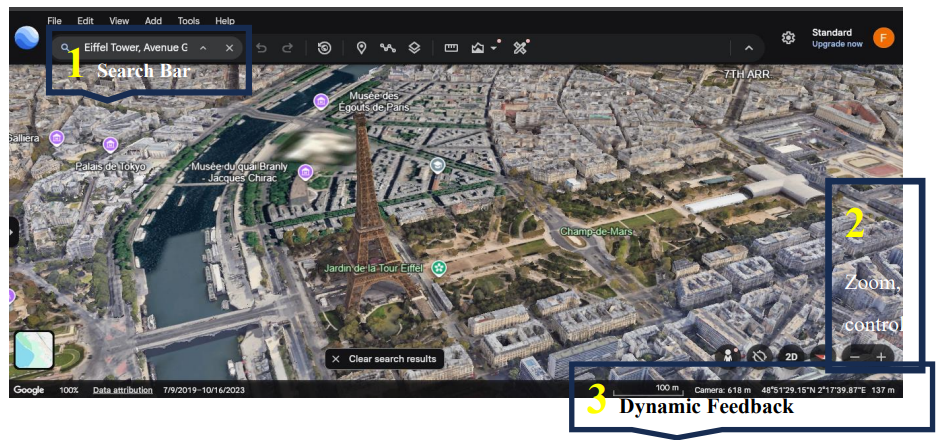
\includegraphics[width=\linewidth]{google_earth.png}
    \caption{Google Earth interface illustrating HCI controls: (1) Search Bar, (2) Zoom Control, and (3) Dynamic Feedback.}
    \label{fig:google_earth_hci}
\end{figure}

\subsection{Search Bar}

A search bar is an interface element that allows users to enter keywords or location names
to find specific places. In the interface, the search bar is used to search for the Eiffel
Tower and quickly navigate to that location.

\subsection{Zoom Controls}

Zoom control allows users to change the viewing scale of the 3D map by zooming in or
out. The plus and minus buttons allow the user to get a closer or wider view of
the Eiffel Tower and its surrounding area.

\subsection{Dynamic Feedback}

Dynamic feedback provides users with information that changes according to their
current interaction or view. The camera information, coordinates, and
altitude displayed at the bottom update according to the user's position and movement in
the 3D environment.

\section{Computer Graphics}
\begin{figure}[htbp]
    \centering
    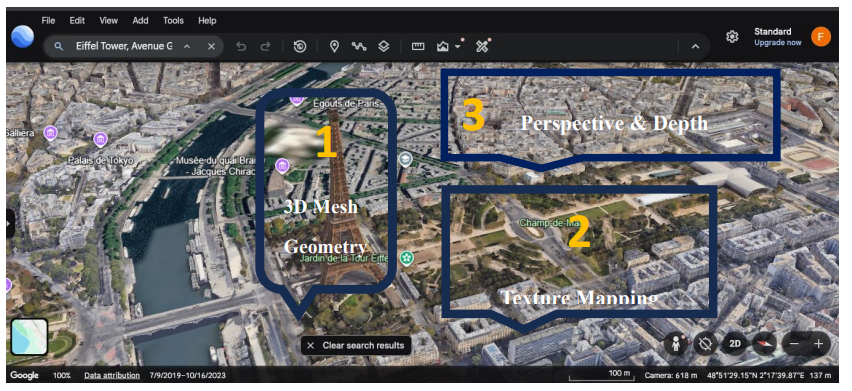
\includegraphics[width=\linewidth]{google_earth_CG.png}
    \caption{Computer Graphics features: (1) 3D Mesh Geometry, (2) Texture Mapping, and (3) Perspective \& Depth.}
    \label{fig:google_earth_cg}
\end{figure}


\subsection{3D Mesh Geometry}

A 3D mesh is the structure made from points, edges, and surfaces
that forms a 3D object. The Eiffel Tower is represented as a 3D
geometric model with height, width, and depth.

\subsection{Texture Mapping}

Texture mapping means applying images or surface details onto a 3D
model to make it look more realistic. Textures and details on buildings and
the environment help them look like real-world objects.

\subsection{Perspective \& Depth}

Perspective projection represents 3D spatial relationships on a 2D screen by rendering distant objects smaller than foreground objects. In the interface, streets, buildings, and ground terrain recede into the distance to provide a natural sense of visual depth.

\section{Reflection Questions}

\subsection{How does the computer graphics quality (e.g realistic lighting or 3D view) help or hinder the user's ability to interact with the software?}
The high-quality Computer Graphics in Google Earth makes interaction easier by
providing a realistic 3D view of buildings, roads, and the environment. Perspective and
depth help users understand distances and navigate the virtual environment more
naturally. However, very detailed graphics may sometimes require more processing
power and can make the software slower on low-performance devices.

\subsection{What is one simple HCI change would you make to improve the user interface?}
I would add clear labels or tooltips to the navigation controls so users can easily
understand what each button does. This would make the interface easier to use, especially
for beginners who are using Google Earth for the first time. It would also reduce
confusion and help users navigate the 3D environment more confidently.

\end{document}